\chapter{Maxwell Equations, Covariance, and Electromagnetic Waves}

We begin exactly where the previous lecture stopped. We already know how electric and magnetic fields act on charged particles; the Lorentz force law tells us that part of the story. The missing half is the reverse question: what determines the fields themselves, and how do charges and currents generate them? In this lecture Leonard Susskind answers that question in a deliberately relativistic way. Maxwell's equations are not introduced merely as a list to memorize, but as field equations to be motivated physically, written covariantly, checked component by component, and then used to derive the existence of light waves. Throughout we work in units with \(c=1\). These notes follow Leonard Susskind closely and are curated by LazyingArt LLC.

\section{From the Lorentz Force to the Missing Field Equations}

The lecture opens by looking backward before it moves forward. Electric and magnetic fields push charged particles around, and the force is proportional to the charge because an uncharged particle does not feel the electromagnetic field at all. In ordinary three-vector language the law is
\begin{align}
\mathbf F = q\bigl(\mathbf E + \mathbf v \times \mathbf B\bigr).
\end{align}
This is the familiar half of electromagnetism: given the fields, we know how matter responds.

\begin{figure}[h]
\centering

\includegraphics[width=0.58\textwidth]{lecture_58_figure_02.png}
\caption{Lorentz force rewritten schematically in field-tensor notation.}
\end{figure}

The board then pivots toward covariant notation. As written there, the second line is only schematic; it suppresses the free force index and the contraction with the four-velocity. The clean covariant statement is
\begin{align}
f^\mu = q\,F^\mu{}_{\nu}\,u^\nu.
\end{align}
Here \(f^\mu\) is the four-force, \(u^\nu\) is the four-velocity, and \(F^{\mu\nu}\) is the antisymmetric electromagnetic field tensor that we will reconstruct shortly. The point of the reminder is not just formal prettiness. Written this way, the Lorentz force law is manifestly the same in every inertial frame.

That is already the standard against which Maxwell's equations will be judged. The missing question is no longer how a charged particle moves in a prescribed field. The missing question is what determines the field itself: what decides whether there is an electric field here, a magnetic field there, or an electromagnetic wave moving through empty space? Those are the equations we now need, and those equations are Maxwell's equations.

As always in this course, the broader issue is relativity. If Maxwell's equations are the theory of light, and if the laws of physics are the same in all inertial frames, then light itself must come out with the same speed in all inertial frames. That is the puzzle Einstein struggled with, and the lecture keeps it in view from the start.

\section{Why Charges Must Affect Fields}

Before writing any field equations, Susskind slows down and asks why charged matter must affect the field at all. A point charge creates an electric field spreading outward from it. A current in a wire creates a magnetic field circulating around the wire. Those are familiar empirical facts, but the lecture wants the deeper logic that makes Maxwell's equations necessary.

The key point is reciprocity sharpened by conservation laws. An electromagnetic wave can hit a charged particle, change its motion, and give it energy. If that can happen, then the influence cannot run only one way. Charged matter must also be able to alter the electromagnetic field. Otherwise energy could appear in the particle without being taken from anywhere.

\subsection{Question \& Answer}

\paragraph{Question.} Why must charged matter act back on the electromagnetic field?

\paragraph{Answer.} Because otherwise energy conservation would fail. If a field can do work on a charge, then a charge must be able to draw energy from the field and modify it. One may call this action and reaction, but the lecture's sharper point is conservation: the field cannot give energy to matter unless matter can affect the field in return.

The lecture then turns that abstract point into a causal picture. Suppose we move a point charge suddenly from one place to another. The field cannot rearrange itself instantaneously throughout all of space. A distant observer is not allowed to see the effect before a light signal could have arrived. Thus the field must rearrange by sending out a disturbance. Near the charge, the rearrangement happens first; farther away, the old field remains until the signal reaches it. If we shake the charge back and forth, the outward-moving disturbance becomes an electromagnetic wave. An antenna is precisely such a device.

The same story can be told for currents. Reverse a current in a wire, and the magnetic field around the wire must reverse as well. But that reversal cannot be known arbitrarily far away in arbitrarily short time. The change in the magnetic field must propagate outward, again as an electromagnetic disturbance. This is the basic physics Maxwell's equations must describe.

\section{Wave Review and Vector-Calculus Review}

Only now does the lecture pause for review. This is not filler. Before Maxwell's equations can be made to produce waves, we first recall what wave equations look like.

Start with a scalar field \(\phi\), a single number attached to each point of spacetime. The relativistic wave equation is
\begin{align}
\partial_\mu \partial^\mu \phi = 0.
\end{align}
With the sign convention used throughout the lecture, this means
\begin{align}
\partial_t^2 \phi - \partial_x^2 \phi - \partial_y^2 \phi - \partial_z^2 \phi = 0.
\end{align}
If the wave moves along the \(z\)-axis, then \(\phi\) depends on \(z\) and \(t\) but not on \(x\) or \(y\), and the equation reduces to
\begin{align}
\partial_t^2 \phi - \partial_z^2 \phi = 0.
\end{align}

\begin{figure}[h]
\centering

\includegraphics[width=0.56\textwidth]{lecture_58_figure_04.png}
\caption{One-dimensional reduction of the wave equation.}
\end{figure}

The lecture emphasizes the two basic traveling-wave solutions,
\begin{align}
\phi = f(z-t), \qquad \phi = g(z+t),
\end{align}
representing right-moving and left-moving profiles. A particularly useful special case is the sinusoidal wave
\begin{align}
\phi(z,t) = \cos\!\bigl(k(z-t)\bigr),
\end{align}
where \(k\) is the wave number. Large \(k\) means short wavelength; small \(k\) means long wavelength. These are exactly the shapes that will later reappear in the electric and magnetic fields themselves.

The lecture then reminds us of the vector operations Maxwell's equations use. For ordinary three-vectors,
\begin{align}
\mathbf a \cdot \mathbf b &= a_x b_x + a_y b_y + a_z b_z,\\
(\mathbf a \times \mathbf b)_x &= a_y b_z - a_z b_y,
\end{align}
with the remaining components obtained by cyclic permutation. For a vector field \(\mathbf A\),
\begin{align}
\nabla \cdot \mathbf A &= \partial_x A_x + \partial_y A_y + \partial_z A_z,\\
(\nabla \times \mathbf A)_x &= \partial_y A_z - \partial_z A_y,
\end{align}
again with cyclic permutation for the other components.

Susskind keeps the geometry in sight. Divergence measures the extent to which a field seems to emanate from somewhere. Curl measures the extent to which it circulates around something. A field of arrows flowing outward from a point suggests divergence; a field winding around a wire suggests curl. These are the operational meanings needed when Maxwell's equations are written down.

\section{Vacuum Maxwell Equations and the Relativity Puzzle}

With that preparation in place, the lecture writes the source-free Maxwell equations, in the order actually used on the board:
\begin{align}
\nabla \times \mathbf E &= -\,\partial_t \mathbf B,\\
\nabla \cdot \mathbf B &= 0,\\
\nabla \times \mathbf B &= \partial_t \mathbf E,\\
\nabla \cdot \mathbf E &= 0.
\end{align}
These are the vacuum Maxwell equations. They describe electric and magnetic fields in the absence of charge density and current density.

Two features are immediately visible. First, the curl equations are almost symmetric under interchange of \(\mathbf E\) and \(\mathbf B\), but not quite: there is an essential sign difference. Second, the divergence equations are asymmetric. The electric field will later acquire a source term \(\rho\), but the magnetic field does not acquire an analogous source term in this lecture, so \(\nabla\cdot\mathbf B=0\).

Susskind briefly points out where sources will eventually go. One will later write
\(\nabla\cdot\mathbf E=\rho\) and \(\nabla\times\mathbf B=\partial_t\mathbf E+\mathbf J\), but for the moment those terms are set aside. This postponement is deliberate. The vacuum equations reveal the covariant structure in its cleanest form.

\subsection{Question \& Answer}

\paragraph{Question.} How can Maxwell's equations be the same in every frame if they imply the same light speed in every frame?

\paragraph{Answer.} That is precisely the relativistic puzzle. If Maxwell's equations are the theory of light, and if those equations are the same in every inertial frame, then every inertial frame must predict the same light speed from them. The resolution is not to patch the wave speed by hand from frame to frame. The resolution is to express the laws in terms of objects with definite Lorentz transformation rules, so that the equations themselves are manifestly frame-independent.

That is why the lecture now turns to the electromagnetic field tensor. The payoff is not elegance by itself. The payoff is that once the equations are written as tensor equations, their invariance is visible, and the constancy of the speed of light follows from the same structure.

\section{The Electromagnetic Field Tensor}

The next move is the central formal pivot of the lecture. The electric and magnetic fields are assembled into a single antisymmetric \(4\times 4\) tensor \(F^{\mu\nu}\). The time coordinate is placed first, so the row and column order is \(t,x,y,z\). The board image fixes the electric entries and the antisymmetric layout.

\begin{figure}[h]
\centering

\includegraphics[width=0.54\textwidth]{lecture_58_figure_03.png}
\caption{Board layout of the electromagnetic field tensor.}
\end{figure}

With the sign convention fixed by the visible board entries, we write
\begin{align}
F^{\mu\nu}=
\begin{pmatrix}
0 & -E_x & -E_y & -E_z\\
E_x & 0 & -B_z & B_y\\
E_y & B_z & 0 & -B_x\\
E_z & -B_y & B_x & 0
\end{pmatrix}.
\end{align}
The diagonal entries vanish because the tensor is antisymmetric, and the entries below the diagonal are the negatives of those above it. The time-space slots contain the electric field; the purely spatial slots contain the magnetic field.

The lecture then introduces a second antisymmetric tensor, the dual tensor \(\tilde F^{\mu\nu}\). We do not need to overdevelop it. What matters is the replacement rule, stated cautiously because Susskind corrects himself while talking through the signs:
\begin{align}
\mathbf E \mapsto -\,\mathbf B, \qquad \mathbf B \mapsto \mathbf E.
\end{align}
With that convention, \(\tilde F^{\mu\nu}\) packages the other half of Maxwell's equations.

At this stage the lecture's rhythm is very clear: write the tensor, inspect its slots, and then ask what covariant first-derivative equations it could possibly satisfy. Since Maxwell's equations contain only first derivatives and should leave one free index, the natural guess is
\begin{align}
\partial_\mu F^{\mu\nu} &= 0,\\
\partial_\mu \tilde F^{\mu\nu} &= 0.
\end{align}
There are four equations in the first line and four in the second, one for each choice of \(\nu\).

Now comes the trust-building step: we check components. For the time component,
\begin{align}
\partial_\mu F^{\mu t}
&= \partial_t F^{tt} + \partial_x F^{xt} + \partial_y F^{yt} + \partial_z F^{zt}\\
&= \partial_x E_x + \partial_y E_y + \partial_z E_z\\
&= \nabla \cdot \mathbf E.
\end{align}
Thus \(\partial_\mu F^{\mu t}=0\) is exactly \(\nabla\cdot\mathbf E=0\).

To stay close to the lecture, it is also useful to check a spatial component. Taking \(\nu=z\),
\begin{align}
\partial_\mu F^{\mu z}
&= \partial_t F^{tz} + \partial_x F^{xz} + \partial_y F^{yz} + \partial_z F^{zz}\\
&= -\,\partial_t E_z + \partial_x B_y - \partial_y B_x\\
&= -\,\partial_t E_z + (\nabla \times \mathbf B)_z.
\end{align}
So \(\partial_\mu F^{\mu z}=0\) is precisely the \(z\)-component of
\begin{align}
\nabla \times \mathbf B = \partial_t \mathbf E.
\end{align}
The other spatial components work the same way. Likewise, \(\partial_\mu \tilde F^{\mu\nu}=0\) packages \(\nabla\cdot\mathbf B=0\) together with \(\nabla\times\mathbf E=-\,\partial_t\mathbf B\).

This is the formal heart of the lecture. Once Maxwell's equations are written as tensor equations, we can see immediately that they are the same in every inertial frame.

\section{From Maxwell to Electromagnetic Waves}

The lecture then pivots from invariance to content: now that Maxwell's equations are written covariantly, what do they actually say? The answer is that they allow wave-like solutions.

We begin with
\begin{align}
\nabla \times \mathbf B = \partial_t \mathbf E
\end{align}
and differentiate once more with respect to time:
\begin{align}
\partial_t^2 \mathbf E = \nabla \times \partial_t \mathbf B.
\end{align}
Now we use the other curl equation,
\begin{align}
\partial_t \mathbf B = -\,\nabla \times \mathbf E,
\end{align}
to eliminate \(\mathbf B\). This gives
\begin{align}
\partial_t^2 \mathbf E = -\,\nabla \times (\nabla \times \mathbf E).
\end{align}
So far the equations still involve the whole vector \(\mathbf E\). The next step, exactly as in the lecture, is to isolate one component, say \(E_x\).

The board algebra is long, but its strategy is simple. The \(x\)-component of the double curl can be reorganized into a clean form:
\begin{align}
\partial_t^2 E_x
&= -\bigl(\nabla \times (\nabla \times \mathbf E)\bigr)_x\\
&= -\,\partial_x(\nabla \cdot \mathbf E)
   + \partial_x^2 E_x + \partial_y^2 E_x + \partial_z^2 E_x.
\end{align}
In vacuum, \(\nabla\cdot\mathbf E=0\), so the first term drops out and we obtain
\begin{align}
\partial_t^2 E_x - \partial_x^2 E_x - \partial_y^2 E_x - \partial_z^2 E_x = 0.
\end{align}
Thus the \(x\)-component of the electric field satisfies the same wave equation that we earlier wrote for the scalar field \(\phi\). This is the exact mathematical payoff Susskind wants. The electric field itself can propagate as a wave.

A simple plane-wave example is now immediate:
\begin{align}
E_x(z,t) = \cos(z-t), \qquad E_y = 0.
\end{align}
This is a right-moving wave along the \(z\)-axis in the lecture's units. It is also polarized: the electric field has been chosen to point along the \(x\)-direction. With the sign convention fixed above, a consistent accompanying magnetic field is
\begin{align}
B_y(z,t) = \cos(z-t), \qquad B_x = B_z = 0.
\end{align}
This explicit \(B_y\) is not copied from the board; it is the clean consequence of the chosen sign convention together with \(\nabla\times\mathbf E=-\,\partial_t\mathbf B\).

\subsection{Question \& Answer}

\paragraph{Question.} Why must the electromagnetic wave be transverse?

\paragraph{Answer.} Because the divergence and curl equations leave no room for a propagating longitudinal component. For a wave depending only on \(z\) and \(t\),
\begin{align}
\nabla \cdot \mathbf E
= \partial_x E_x + \partial_y E_y + \partial_z E_z
= \partial_z E_z.
\end{align}
In vacuum this must vanish, so
\begin{align}
\partial_z E_z = 0.
\end{align}
Therefore \(E_z\) can at most be a constant. A constant field is not part of the wave profile, so the wave part of the \(z\)-component must be absent.

Now look at the curl. If \(E_x(z,t)\) is nonzero while \(E_y=0\) and the wave part of \(E_z\) vanishes, then the only nonzero component of \(\nabla\times\mathbf E\) lies along \(y\). But \(\nabla\times\mathbf E=-\,\partial_t\mathbf B\), so the magnetic field itself must point along \(y\). Hence
\begin{align}
\mathbf E \perp \hat z, \qquad \mathbf B \perp \hat z, \qquad \mathbf E \perp \mathbf B.
\end{align}
That is the transversality of electromagnetic radiation. The electric field, the magnetic field, and the direction of propagation are mutually perpendicular.

\begin{remark}
The next frame is kept because it preserves the board geometry of the wave, even though its subtitle metadata is mismatched. Its evidentiary value here is visual: it belongs to the wave-and-polarization discussion, not to the anti-symmetric-matrix discussion suggested by the subtitle timing.
\end{remark}

\begin{figure}[h]
\centering

\includegraphics[width=0.48\textwidth]{lecture_58_figure_05.png}
\caption{Board sketch of a transverse wave propagating along \(z\).}
\end{figure}

\begin{figure}[h]
\centering
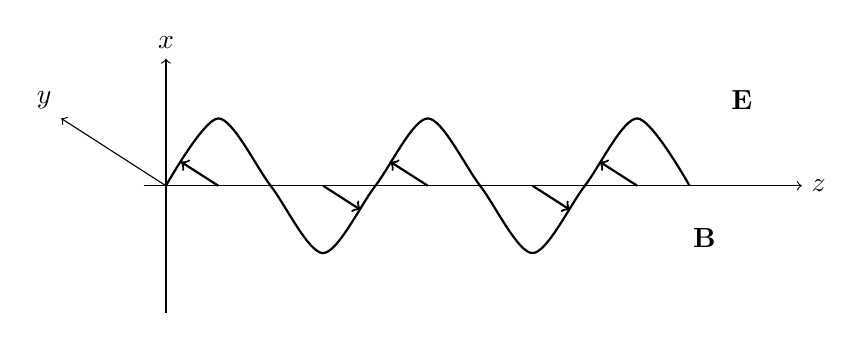
\begin{tikzpicture}[scale=0.95]
\draw[->] (-0.3,0) -- (8.5,0) node[right] {$z$};
\draw[->] (0,-1.7) -- (0,1.7) node[above] {$x$};
\draw[->] (0,0) -- (-1.4,0.9) node[above left] {$y$};

\draw[thick] plot[smooth] coordinates {
(0.0,0.0)
(0.7,0.9)
(1.4,0.0)
(2.1,-0.9)
(2.8,0.0)
(3.5,0.9)
(4.2,0.0)
(4.9,-0.9)
(5.6,0.0)
(6.3,0.9)
(7.0,0.0)
};

\draw[->,thick] (0.7,0.0) -- (0.2,0.32);
\draw[->,thick] (2.1,0.0) -- (2.6,-0.32);
\draw[->,thick] (3.5,0.0) -- (3.0,0.32);
\draw[->,thick] (4.9,0.0) -- (5.4,-0.32);
\draw[->,thick] (6.3,0.0) -- (5.8,0.32);

\node at (7.7,1.15) {$\mathbf E$};
\node at (7.2,-0.7) {$\mathbf B$};
\end{tikzpicture}
\caption{A clean reconstruction of the transverse electromagnetic-wave geometry: propagation along \(z\), electric field along \(x\), magnetic field along \(y\).}
\end{figure}

This is the lecture's physical climax. Maxwell's equations imply electromagnetic waves, those waves move with speed \(1\) in the chosen units, and their electric and magnetic fields are transverse and polarized. Because the equations themselves are the same in every frame, these structural properties belong to every inertial observer.

\section{Restoring Sources: Charge, Current, Continuity, and Covariance}

Only after the vacuum story is clear does the lecture restore what had been postponed: charge density and current density. The Maxwell equations become
\begin{align}
\nabla \cdot \mathbf E &= \rho,\\
\nabla \cdot \mathbf B &= 0,\\
\nabla \times \mathbf E &= -\,\partial_t \mathbf B,\\
\nabla \times \mathbf B &= \partial_t \mathbf E + \mathbf J.
\end{align}
Here \(\rho\) is the charge density and \(\mathbf J\) is the current density.

The charge density is defined by
\begin{align}
\rho = \frac{dQ}{dV},
\end{align}
so that the charge in a region \(V\) is
\begin{align}
Q_V = \int_V \rho\,dV.
\end{align}
The lecture emphasizes the continuum approximation: in reality space may contain many individual charges, but if we coarse-grain over sufficiently small regions we may treat charge as a continuous density field.

The density \(\rho\) can depend on time as well as position, because charge can move. But it cannot change arbitrarily. The total amount of charge in the universe is conserved, and the lecture immediately strengthens that statement. Charge is not allowed simply to disappear here and reappear there with nothing in between. If charge leaves one region and appears in another, there must be a flow of charge connecting the two.

\subsection{Question \& Answer}

\paragraph{Question.} Why is charge conservation stronger than the statement that total charge is constant?

\paragraph{Answer.} Because global constancy by itself would still allow absurd behavior: charge could vanish on Earth and reappear on Mars without anything happening in between. The lecture forbids that. Charge may move from one place to another only by flowing through the intervening space. That stronger, local form of conservation is what leads to current density and to the continuity equation.

To describe such flow, take an infinitesimal oriented surface element \(d\boldsymbol{\sigma}\). The charge per unit time passing through it is
\begin{align}
\frac{dQ}{dt} = \mathbf J \cdot d\boldsymbol{\sigma}.
\end{align}
This is why current is a vector. Its magnitude is charge per unit area per unit time, and its direction is the direction in which charge flows.

Now fix a spatial region \(V\) with outward-pointing boundary element \(d\boldsymbol{\sigma}\). If net current flows outward through the boundary, the charge inside must decrease. Thus
\begin{align}
\frac{dQ_V}{dt} = -\oint_{\partial V} \mathbf J \cdot d\boldsymbol{\sigma}.
\end{align}
Since \(Q_V=\int_V \rho\,dV\), we also have
\begin{align}
\frac{dQ_V}{dt} = \int_V \partial_t \rho\,dV.
\end{align}
Combining the two,
\begin{align}
\int_V \partial_t \rho\,dV = -\oint_{\partial V} \mathbf J \cdot d\boldsymbol{\sigma}.
\end{align}

At this point the lecture invokes Gauss's theorem, also called the divergence theorem:
\begin{align}
\oint_{\partial V} \mathbf A \cdot d\boldsymbol{\sigma}
= \int_V (\nabla \cdot \mathbf A)\,dV.
\end{align}
Applying it to \(\mathbf J\) gives
\begin{align}
\int_V \partial_t \rho\,dV
= -\int_V (\nabla \cdot \mathbf J)\,dV.
\end{align}
If this holds for every region \(V\), then the integrands themselves must agree, and we obtain
\begin{align}
\partial_t \rho + \nabla \cdot \mathbf J = 0.
\end{align}
This is the continuity equation, the local form of charge conservation.

Now the relativistic packaging becomes natural. The four quantities \(\rho, J_x, J_y, J_z\) form the four-current
\begin{align}
J^\mu = (\rho, J_x, J_y, J_z),
\end{align}
and the continuity equation becomes
\begin{align}
\partial_\mu J^\mu = 0.
\end{align}

The sourced Maxwell equations themselves then collapse into a single covariant equation:
\begin{align}
\partial_\mu F^{\mu\nu} = J^\nu.
\end{align}
For \(\nu=t\), the right-hand side is \(J^t=\rho\), so the equation becomes
\begin{align}
\nabla \cdot \mathbf E = \rho.
\end{align}
For spatial \(\nu\), it becomes
\begin{align}
\nabla \times \mathbf B = \partial_t \mathbf E + \mathbf J.
\end{align}
The other half of Maxwell's equations remains
\begin{align}
\partial_\mu \tilde F^{\mu\nu} = 0.
\end{align}

So the return of sources does not spoil covariance. On the contrary, it completes it. Charges and currents enter as a four-vector, and the field equations remain tensor equations. The way fields act on matter is Lorentz invariant, and the way matter generates fields is Lorentz invariant as well.

\section{Summary}

The lecture has a very definite arc. We begin with the Lorentz force law and identify the missing half of the subject: not how fields act on matter, but how matter determines fields. Maxwell's equations answer that question. In vacuum they can be written as the covariant equations \(\partial_\mu F^{\mu\nu}=0\) and \(\partial_\mu \tilde F^{\mu\nu}=0\), and from them we derive wave equations for the field components themselves. A plane-wave solution then shows that electromagnetic radiation is transverse and polarized, with \(\mathbf E\), \(\mathbf B\), and the direction of propagation mutually perpendicular.

Finally, when charges and currents are restored, the continuity equation and the four-current \(J^\mu\) lead to the sourced covariant equation \(\partial_\mu F^{\mu\nu}=J^\nu\). That is the closing point Susskind wants to leave with us: electromagnetism can be written entirely in Lorentz-covariant form, and because those same laws imply waves moving with speed \(c\), light travels with the same speed in every inertial frame.